%% Files that are needed for LaTeX processing (style + inputs) are available
%% relative to the download place in the directory ../inputs, the images in
%% ../img

\documentclass[compress]{beamer}

\usepackage[utf8]{inputenc}
\mode<presentation>{
   \usetheme{Boadilla}
   \hypersetup{pdfpagemode=FullScreen}
}
\setbeamertemplate{navigation symbols}{}

\usepackage{debian-links}

\title{Debian Teams Activity Metrics}

\author{Andreas Tille \& Sukhbir Singh}

%\institute{\Debian}
\institute{\link{http://www.debconf.org/debconf11/}{DebConf 11}}

\date{Banja Luka, July 29, 2011}

\begin{document}

\begin{frame}
  \titlepage
\end{frame}

\section{Short historical introduction}

\begin{frame}
  \frametitle{Motivation}

  \begin{itemize}
     \item Who is inside the team?
     \item Who left the team?
     \item Does a team have enough members?
     \item Is the team growing or shrinking?
  \end{itemize}
\end{frame}

\begin{frame}
  \frametitle{Quite simple start: Mailing list activity}
      \begin{center}
        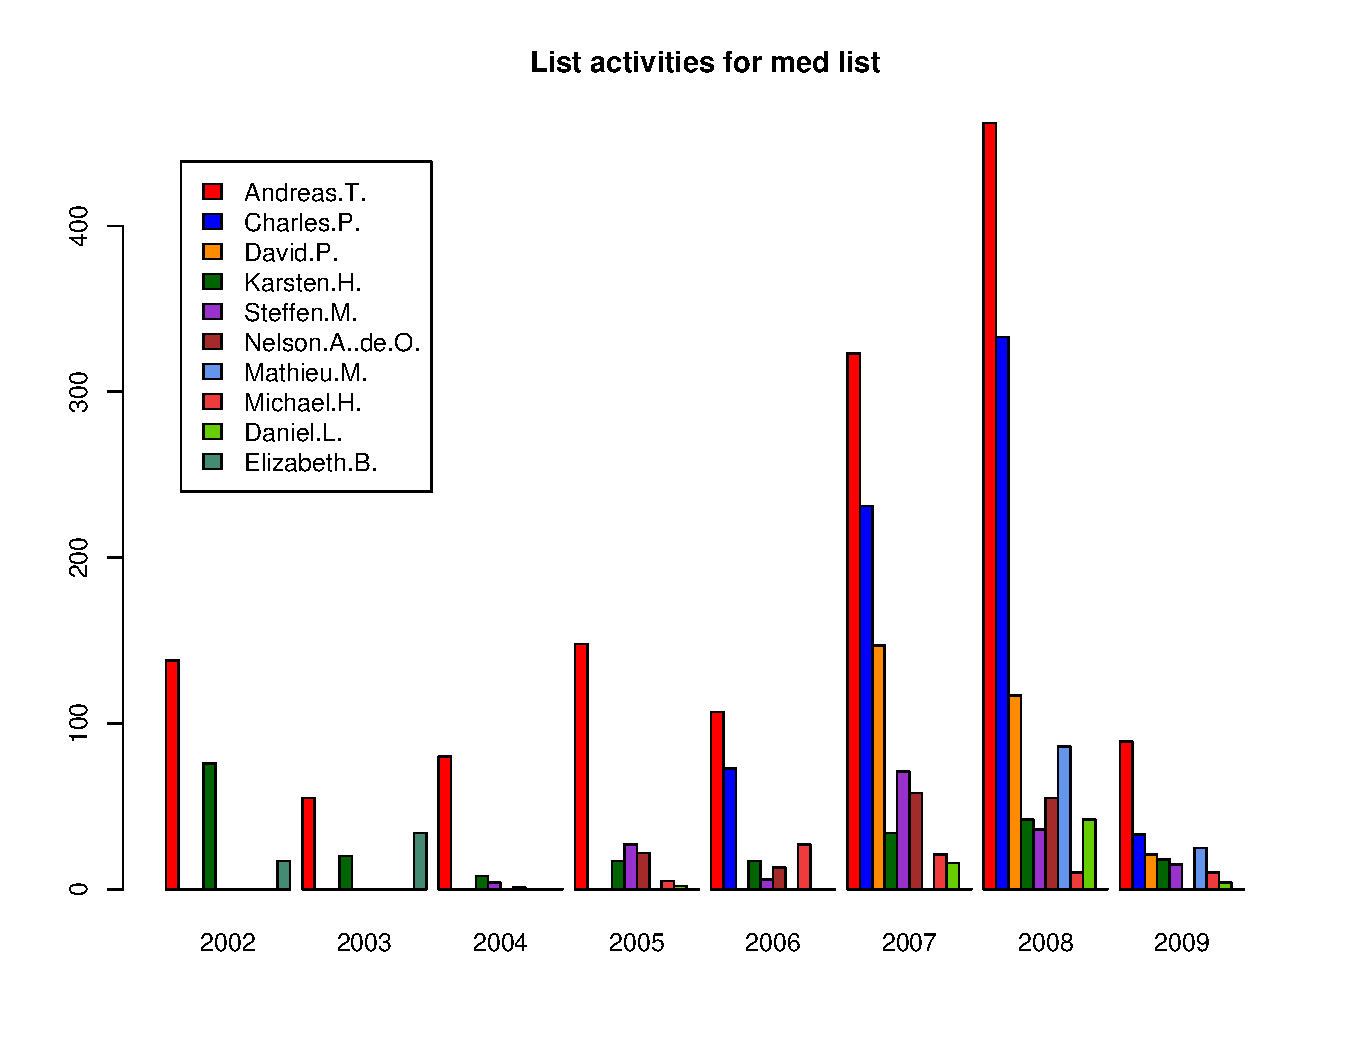
\includegraphics[width=0.9\textwidth]{authorstat_med}
      \end{center}

\end{frame}

\begin{frame}
  \frametitle{Enhancing the observation needed}
  \begin{itemize}
    \item We do not only want to know who is ``chatting''
    \item There should be a ``fair'' evaluation
    \item More flexibility
    \item Technical enhancements
  \end{itemize}
\end{frame}


\section{GSoC Project}

\begin{frame}
  \frametitle{Additional channels / means % FIXME
              to consider
             }
  \begin{itemize}
    \item VCS commits
    \item Uploaded packages
    \item IRC activity % FIXME ... just got this idea when writing ...
    \item ... you suggest!
  \end{itemize}
\end{frame}

\begin{frame}
  \frametitle{Measure of Communication Activity}

  \begin{itemize}
     \item Every project has a mailing list
     \item We measure who are the most active contributors
     \item Quantity is not the only metric because quality matters 
     \item We handle spam by filtering it
  \end{itemize}

\end{frame}

\begin{frame}
 \frametitle{Metrics for Measuring Communication Activity}

 \begin{itemize}
    \item Frequency of posting 
    \item Message body metrics 
    \begin{itemize}
        \item the raw length of the message body
        \item the length of the body excluding 

        \begin{itemize}
            \item blank lines
            \item blank lines and quotes
            \item blank lines, quotes and signatures
        \end{itemize}
    
    \end{itemize}

 \end{itemize}
\end{frame}

\end{document}
